\section{Théorème de Pythagore}
\subsection{Vocabulaire du triangle}
\begin{voc}
    \begin{itemize}
        \item Un triangle qui possède un angle droit est un triangle \answer{rectangle}.
        \item Le côté opposé à l'angle de droit est appelé \answer{hypoténuse}. C'est
            le plus \answer{grand} côté du triangle.
    \end{itemize}
\end{voc}
\begin{exe}
    \begin{minipage}{0.38\textwidth}

        \begin{tikzpicture}[line cap=round,line join=round,>=triangle
            45,scale=0.8]
            \begin{axis}[
                x=1.0cm,y=1.0cm,
                axis lines=none,
                xmin=1.5,
                xmax=10.0,
                ymin=0.8,
                ymax=5.5,
                ]
                \clip(1.5,0.8) rectangle (10.,5.5);
                \fill[line width=2.pt,color=zzttqq,fill=zzttqq,fill opacity=0.10000000149011612] (2.0969157848306166,0.9903084215169384) -- (4.0969157848306175,4.990308421516938) -- (9.472915784830617,2.3023084215169374) -- cycle;
                \draw[line width=2.pt,color=qqwuqq,fill=qqwuqq,fill opacity=0.10000000149011612] (3.9459520616007877,4.688380975057279) -- (4.247879508060447,4.537417251827449) -- (4.398843231290277,4.839344698287109) -- (4.0969157848306175,4.990308421516938) -- cycle; 
                \draw [line width=2.pt,color=zzttqq] (2.0969157848306166,0.9903084215169384)-- (4.0969157848306175,4.990308421516938);
                \draw [line width=2.pt,color=zzttqq] (4.0969157848306175,4.990308421516938)-- (9.472915784830617,2.3023084215169374);
                \draw [line width=2.pt,color=zzttqq] (9.472915784830617,2.3023084215169374)-- (2.0969157848306166,0.9903084215169384);
                \begin{scriptsize}
                    \draw[color=ududff] (1.9174947510970175,1.504331168562242) node {$E$};
                    \draw[color=ududff] (4.208962956531576,5.291618896988809) node {$D$};
                    \draw[color=xdxdff] (9.58754804984325,2.602326350332969) node {$F$};
                \end{scriptsize}
            \end{axis}
        \end{tikzpicture}

    \end{minipage}
    \begin{minipage}{0.60\textwidth}
        \begin{itemize}
            \item DEF est un triangle rectangle en D.
            \item \text{[EF]} est l'hypoténuse de DEF : c'est le plus grand côté.
            \item Les autres côtés [DF] et [DE] sont perpendiculaires.
        \end{itemize}
    \end{minipage}

\end{exe}

\subsection{Enoncé du Théorème}

\begin{theorem}

    \begin{tikzpicture}[scale=1.25]%,cap=round,>=latex]

        \coordinate [label=left:$C$] (A) at (-1.5cm,-1.cm);
        \coordinate [label=right:$A$] (C) at (1.5cm,-1.0cm);
        \coordinate [label=above:$B$] (B) at (1.5cm,1.0cm);
        \draw (A) -- node[above] {$a$} (B) -- node[right] {$c$} (C) -- node[below] {$b$} (A);

        \draw (1.25cm,-1.0cm) rectangle (1.5cm,-0.75cm);
        \node[text width=9cm, anchor=west, right] at (3,0){
            Dans le triangle ABC rectangle en A, d'après le \bb{théorème de
            Pythagore} on a : 
        \begin{equation*}
            BC^2=AB^2+AC^2
        \end{equation*}
        ou encore :
        $$a^2=b^2+c^2$$
        On dit que \it{le carré de l'hypoténuse est égal à la somme des carrés des
        deux autres côtés}.
        };
    \end{tikzpicture}
\end{theorem}

\subsection{Application : Calculer la longueur d'un côté quand on en connait
deux}
\subsubsection{Calculer la longueur de l'hypoténuse}
\begin{exe}
    \begin{minipage}{0.48\textwidth}

    Soit DEF un triangle rectange en D tel que DE=4cm et DF=4cm. 

        Calculer la longueur de [EF].
    \end{minipage}
    \hfill
    \begin{minipage}{0.48\textwidth}

    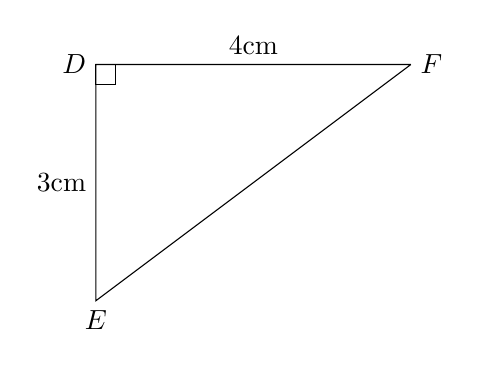
\begin{tikzpicture}[scale=1]%,cap=round,>=latex]

        \coordinate [label=left:$D$] (C) at (-2cm,+1.5cm);
        \coordinate [label=below:$E$] (B) at (-2cm,-1.5cm);
        \coordinate [label=right:$F$] (A) at (+2cm,1.5cm);
        \draw (A) --  (B) -- node[left] {3cm} (C) -- node[above] {4cm} (A);

        \draw (-2cm,1.5cm) rectangle (-1.75cm,1.25cm);
    \end{tikzpicture}
    \end{minipage}
    Etape 1: On rédige le théorème de Pythagore.

    Dans le triangle DEF rectangle en D, d'après le théorème de Pythagore on a: 
    \begin{align*}
        EF^2&=\answer{DE^2+DF^2} \\
        EF^2&=\answer{3^2+4^2} \\
        EF^2&=\answer{9+16=25}
    \end{align*}
    Donc EF=\answer{$\sqrt{25} = 5cm$}

\end{exe}
\subsubsection{Calculer la longueur d'un côté de l'angle droit}

\begin{exe}
    \begin{minipage}{0.48\textwidth}

    Soit DEF un triangle rectange en D tel que DE=5cm et EF=8cm. 

        Calculer la longueur de [DF].
    \end{minipage}
    \hfill
    \begin{minipage}{0.48\textwidth}

        \begin{tikzpicture}[line cap=round,line join=round,>=triangle
            45,scale=0.8]
            \begin{axis}[
                x=1.0cm,y=1.0cm,
                axis lines=none,
                xmin=1.5,
                xmax=10.0,
                ymin=0.8,
                ymax=5.5,
                ]
                \clip(1.5,0.8) rectangle (10.,5.5);
                \fill[line width=2.pt,color=zzttqq,fill=zzttqq,fill opacity=0.10000000149011612] (2.0969157848306166,0.9903084215169384) -- (4.0969157848306175,4.990308421516938) -- (9.472915784830617,2.3023084215169374) -- cycle;
                \draw[line width=2.pt,color=qqwuqq,fill=qqwuqq,fill opacity=0.10000000149011612] (3.9459520616007877,4.688380975057279) -- (4.247879508060447,4.537417251827449) -- (4.398843231290277,4.839344698287109) -- (4.0969157848306175,4.990308421516938) -- cycle; 
                \draw [line width=2.pt,color=zzttqq] (2.0969,0.99)-- (4.09,4.99);
                \draw [line width=2.pt,color=zzttqq] (4.0969,4.99)-- (9.47,2.30);
                \draw [line width=2.pt,color=zzttqq] (9.4729,2.30)-- (2.09,0.99);
                \begin{scriptsize}
                    \draw[color=ududff] (1.9174947510970175,1.504331168562242) node {$E$};
                    \draw[color=ududff] (4.208962956531576,5.291618896988809) node {$D$};
                    \draw[color=xdxdff] (9.58754804984325,2.602326350332969) node {$F$};
                \end{scriptsize}
            \end{axis}
        \end{tikzpicture}

    \end{minipage}
    Etape 1: On rédige le théorème de Pythagore.

    Dans le triangle DEF rectangle en D, d'après le théorème de Pythagore on a: 
    \begin{align*}
        EF^2&=DE^2+DF^2 \\
        8^2&=5^2+DF^2 \\
        DF^2&=\answer{8^2-5^2} \\
        DF^2&=\answer{64 - 25 = 39}
    \end{align*}
    Donc DF=\answer{$\sqrt{39} \approx 6.2cm$}
\end{exe}

\subsection{Application : Montrer qu'un triangle n'est pas rectangle}
\begin{exe}
    On peut se servir du théorème de Pythagore pour \bb{démontrer qu'un triangle
    n'est pas rectangle}. 
    \newline
    \newline
    Considérons un triangle HJK tel que 
    $$HJ=3cm\hspace{2cm}JK=5,6cm\hspace{2cm}HK=4,2cm$$
    \bb{Le plus grand côté} est JK. Calculons alors $JK^2$ et $HJ^2+HK^2$ pour
    vérifier si l'égalité de Pythagore est vérifiée.\\
    \begin{minipage}{0.48\textwidth}
        \begin{align*}
            JK^2&=\answer{5.6^2}\\
            &=\answer{31.36}\\
        \end{align*}
    \end{minipage}
    \hfill
    \begin{minipage}{0.48\textwidth}
        \begin{align*}
            HK^2+HJ^2&=\answer{4.2^2+3^2}\\
            &=\answer{26.64}\\
        \end{align*}
    \end{minipage}\\
    Or $\answer{31.36} \neq \answer{26.64}$ donc HJK ne respecte pas l'égalité
    de Pythagore et \bb{n'est donc pas un triangle
    rectangle}.
\end{exe}
